\section{Experimental Studies}
\label{sec:eval}
We conduct several experiments to evaluate the performance of our
model by comparing with the state-of-the-art techniques.
First, we present the experimental setup in \secref{sec:data} and
the model selection strategy in \secref{sec:para};
Then, we apply our model to the three applications.
We show the accuracy and efficiency of
our recommendation algorithm in POI recommendation in \secref{sec:poirec}
and explore the reason of making a POI recommendation
in \secref{sec:reason}.
After that, we show the accuracy of user recommendation
in \secref{sec:userrec}.
Finally, we analyze the aspect satisfaction in regions in \secref{sec:satisfy}
and discuss the quality of topical
regions in \secref{sec:regions}.

\subsection{Experimental Setup}
\label{sec:data}
We collect data from two different cities in Yelp,
which hosts
hundreds of thousands of user reviews and ratings for POIs.
%We do not use rating in our model because some sites like
%Foursquare do not have ratings. Our model is more general
%than rating dependent systems, so that can be applied
%to every sites which provides user review or tips.
%Ratings in our experiment is used for evaluating
%our recommendation results.
One of our datasets is from Yelp's Challenge
Dataset\footnote{http://www.yelp.com.sg/dataset\_challenge/}, which
contains 11,537 POIs and 43,873 users from Phoenix at
the time of data collection. We remove users
who wrote fewer than 2 reviews and POIs without any reviews
after filtering the users. This preprocessing results
in a dataset containing 11,359 POIs and 21,908 users.
We crawl the other dataset from Yelp Singapore, and
remove users and POIs without any reviews.
The resulting Singapore dataset
contains 8,846 POIs and 1,654 users.
The statistics of the two
datasets is shown in \tabref{tab:data}.
For each dataset, we hold out the recent
10\% reviews of each user for tuning and 10\% for testing, respectively,
and use the remaining 80\% data as training set. In
the tuning and test data, we generate the ground truth,
i.e., whether a user likes the POI or not, by checking
how the user rates to that POI. When the user rates
more than 3.5 stars, we consider that she likes the POI and
put the user-POI pair into the set of ground truth.

\begin{table}[th]
\centering
%\scriptsize
\caption{Statistics of the two datasets}
\begin{tabular}{l|r|r}
\hline
& Phoenix & Singapore\\
\hline
\#POIs & 11,359 & 8,846 \\
\hline
\#Users & 21,908 & 1,654 \\
\hline
\#Reviews & 215,837 & 20,248 \\
\hline
\#Reviews per user & 4.92  & 12.40\\
\hline
\#Reviews per POI & 18.71 & 2.36\\
\hline
\end{tabular}
\label{tab:data}
\end{table}

We run all experiments on a machine with
Intel Xeon E5-2680 (2.8 Ghz) 10-cores CPU and 64GB memory.
We deploy the training program on 8 cores of the CPU and
train the SAR models on Singapore
and Phoenix datasets with the same settings as in \secref{sec:para}.
The training time of Singapore data is 33.74 minutes and the
Phoenix data is 965.61 minutes.

\subsection{Model Selection}
\label{sec:para}
In our model, we have two free parameters: number of
aspects $A$ and number of topical regions $R$, and a
tunable parameter $\lambda$. To find a proper value of
$A$ and $R$, we use Bayesian Information Criterion (BIC)
which is usually used for model selection.
%As we know, the
%more parameters we have in the model, the better our
%model can probably fit the training data. To handle the
%overfitting problem,
%BIC gives penalty to the number of parameters.
BIC is defined as: $BIC=-2L+Kln(N)$,
where $L$ is the likelihood of the model, $K$ is the number of parameters
and $N$ is the scale of the corpus. In our scenario, $K$ is
$A\times R$, while $N$ is the number of review sentences.
%We choose the value
%of $A$ and $R$ with low BIC score.
%The BIC scores of different $A$
%and $R$ are shown in \figref{fig:bic}.
We set the default value of parameter $\lambda$ to 0.6,
%The BIC score of the model is very close in different number of
%free parameters. As the number of parameters increases, the penalty
%term $Kln(N)$ becomes larger. But model with more parameters can
%fit the data better which results in a higher likelihood. We
and choose $A$,$R$ which achieve lowest BIC in the tuning set of each dataset.
In the Phoenix data, the lowest BIC appears when $R=80$
and $A=30$.
In the Singapore data, smaller number of aspects and regions are preferred
because Singapore is smaller than Phoenix. We set $R=40$ and $A=20$ for
Singapore data.

%\begin{figure}[th]
%\centering
%\begin{subfigure}[t]{0.47\columnwidth}
%\centering
%\epsfig{file=fig/bic_p.eps,width=\columnwidth}
%\caption{Phoenix}
%\end{subfigure}
%\begin{subfigure}[t]{0.47\columnwidth}
%\centering
%\epsfig{file=fig/bic_s.eps,width=\columnwidth}
%\caption{Singapore}
%\end{subfigure}
%\caption{Model Selection by BIC}
%\label{fig:bic}
%\end{figure}

%\subsubsection{Parameter Tuning}
%We have one tunable parameters $\lambda$ in our model.
%We tune $\lambda$ by empirically comparing the effect
%of different $\lambda$ on the MAP score in POI recommendation
%(See \figref{fig:lambda}).
%Both of the two datasets have
%best MAP scores when $\lambda=0.6$, which means the
%aspect and sentiment words are more frequently used in a review than
%region words.
%
%\begin{figure}[th]
%%\begin{subfigure}[t]{0.49\columnwidth}
%%\centering
%%\epsfig{file=fig/kappa_all_map.eps,width=\columnwidth}
%%\caption{Effect of $\kappa$ in All-category POI recommendation}
%%\end{subfigure}
%%\begin{subfigure}[t]{0.49\columnwidth}
%\centering
%\epsfig{file=fig/lambda_all_map.eps,width=0.7\columnwidth}
%\caption{Effect of $\lambda$ in All-category POI recommendation}
%%\end{subfigure}
%%\begin{subfigure}[t]{0.49\columnwidth}
%%\centering
%%\epsfig{file=fig/kappa_all_recall.eps,width=\columnwidth}
%%\caption{Effect of $\kappa$ in Single-category POI recommendation}
%%\end{subfigure}
%%\begin{subfigure}[t]{0.49\columnwidth}
%%\centering
%%\epsfig{file=fig/lambda_all_recall.eps,width=\columnwidth}
%%\caption{Effect of $\lambda$ in Single-category POI recommendation}
%%\end{subfigure}
%%\begin{subfigure}[t]{0.49\columnwidth}
%%\centering
%%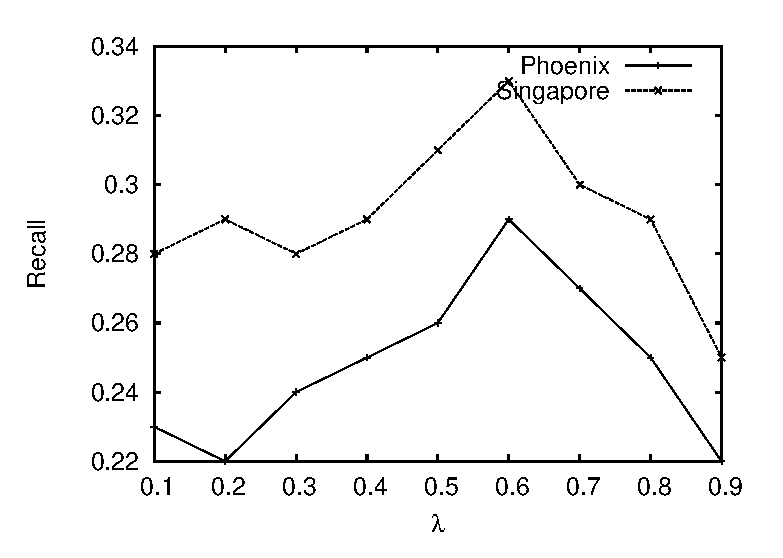
\epsfig{file=fig/lambda.eps,width=\columnwidth}
%%\caption{Effect of $\kappa$ in User recommendation}
%%\end{subfigure}
%%\begin{subfigure}[t]{0.49\columnwidth}
%%\centering
%%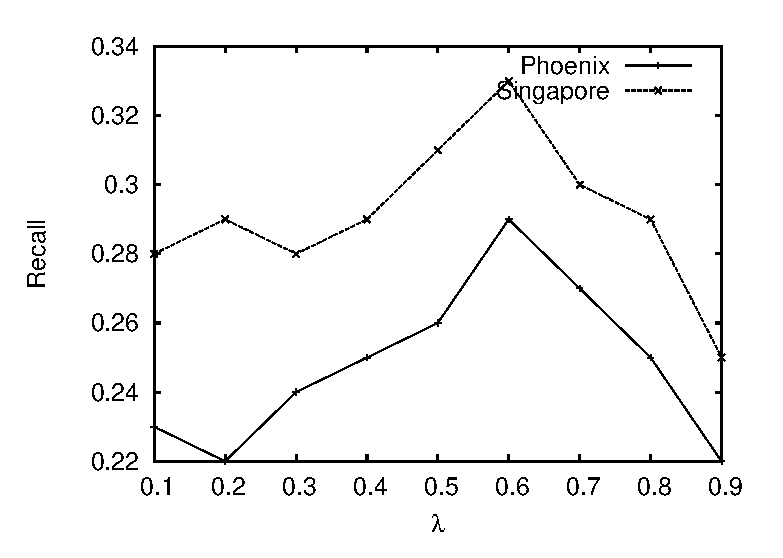
\epsfig{file=fig/lambda.eps,width=\columnwidth}
%%\caption{Effect of $\lambda$ in User recommendation}
%%\end{subfigure}
%\caption{Parameter Tuning}
%\label{fig:lambda}
%\end{figure}

%\subsection{Baselines}
%\label{sec:base}
%%We apply our model to POI recommendations and user recommendations to
%%show the effectiveness of modeling the interdependency
%%of aspect, sentiment and region.
%We compare our model to two existing POI recommendation
%methods, which can be applied to our dataset. One of them is typical
%user based collaborative filtering(CF) while the other is a state-of-the-art
%Geo-Social based POI recommendation model proposed by Ye et al. \cite{YeGeoSocial:2011}.
%%Ye's model is an improvement of CF by incorporating the spatial and social
%%information.
%Since social relation is not our main concern in this paper
%and we do not have social network in our dataset,
%we only use the check-in and geographical information
%of Ye's model, and
%we set the parameter $\alpha=0.3$ for
%Phoenix and $\alpha=0.7$ for Singapore,
%which achieve the best MAP on the tuning set.

\subsection{POI recommendation}
\label{sec:poirec}
First, we introduce several existing methods for competition and
the evaluation metrics. Then, we compare with
the state-of-the-art baselines for both all-category and single-category
recommendation. Finally, we evaluate the efficiency of our
recommendation algorithm.

\subsubsection{Recommendation Methods}
We compare our model to five POI recommendation techniques.
\begin{itemize}
\item \textbf{CF}: User-based collaborative filtering model.
\item \textbf{GCF}: A collaborative filtering model incorporating \\
geographical influence \cite{YeGeoSocial:2011}.
\item \textbf{W3}: A topic model with personalized regions \cite{YuanW4:2013}.
\item \textbf{STM}: A topic model with global regions \cite{HuSTM:2013}.
\item \textbf{EFM}: A matrix factorization based explicit factor model 
which extracts aspects and sentiment from reviews, and  models
the relation among user, item, aspect and sentiment for recommendation \cite{ZhangYF14}.
\item \textbf{GEFM}: We multiply the EFM rating score with a geographical score given by
$exp\{-dist(u,l)\}$. Function $dist(u,l)$ is the average distance from POI $l$ to POIs that the user
has visited.
\end{itemize}

\subsubsection{Evaluation Metrics}
%Both POI and user recommendation result in a set of rank list
%of items (POI or user). Therefore, we can evaluate them in the same
%manner.
Evaluating a recommended list has two ways: one of
them is how many true results are hit by the list and the other is
how similar the resulting rank and the ground truth rank are.
Therefore, we use two kinds of metrics to measure the performance of our model
and the peers. These metrics are: 1) the precision and recall for
the top N items, namely \emph{Precision@N} and \emph{Recall@N}, respectively.
%It is computed by averaging the
%recalls of the recommendation results for all users. For each user,
%the recall is computed as the number of the ground truth in the
%top $N$ items divided by total number of ground truths.
We investigate
$N=5$ and $N=10$ because the top few results are most impressive
to users. %and usually $N$ less than 10 is proper to be shown in the
%mobile devices.
2) \emph{Mean Average Precision} (MAP)
which is used to show the correctness of a rank list according
to the position of true results in the list.
If the true results are ranked high in the list, the list is probably
a good recommendation result.

%MAP is defined as \equref{eq:map}
%\begin{equation}
%MAP=\frac{\sum_{i}^{N}{\frac{\sum_{L_k\in G_i}{P(k)}}{|G_i|}}}{N},
%\label{eq:map}
%\end{equation}
%where $N$ is the total number of rank lists, i.e. number of users in POI
%recommendation and number of POIs in user recommendation; $G_i$
%is the set of ground truths of list $i$; $L_k$ is the $k$-th item;
%$P(k)$ is the precision of the
%top $k$ items in the resulting rank list.

\subsubsection{All-Category POI Recommendation}
The result
is shown in \figref{fig:poi}.
All results reported in this section pass t-test with
p-value$<0.01$, which means the improvements are significant.
%Our SAR model has one tunable parameters $\lambda$. We tune
%the value of $\lambda$ by empirically comparing the effect
%of different $\lambda$ on the MAP score in POI recommendations.
%In the following experiments, we set $\lambda=0.6$ for
%both datasets.
Our SAR model outperforms
the best peer by 33\% , 34\% and 61\% in terms of
Precision@10, Recall@10 and MAP, respectively
on the Phoenix dataset, while 59\% ,
90\% and 62\% in terms of
Precision@10, Recall@10 and MAP, respectively
on the Singapore dataset.

Among the baseline methods, CF and EFM do not
consider geographical information, which limits
the performance of these two methods.
Compared to CF, EFM performs better because it
explores the user preferences on aspect level.
GEFM performs 
the best among the baselines, but still worse 
than SAR because it does not model the interdependencies.
W3 has lower performance than GCF model in some cases 
because it learns small personalized regions for 
users who have limited number of
visiting records, which leads to overfitting.
%However, if a
%user visits a small number of POIs (e.g., 1 or 2),
%the regions learnt by the model would be constrained
%in a small area. Therefore, POIs in other regions
%have rare chance to be recommended.
STM performs
worst because it estimates
the probability $p(l|r)$ by the probability density
function of Gaussian distribution without any
normalization. The Gaussian distribution in STM
overwhelms the other probabilities (i.e.,
the preferences of the user). GCF
incorporates the graphical information into the model of CF.
However, without considering
the content of the reviews,
GCF cannot reveal user's preferences
on aspect level.

%User-based CF has two drawbacks
%in POI recommendations. First, a user shows her
%interest on the POI by posting a review on it.
%Even though the user writes a negative review on
%the POI, the system identify the POI as the user's
%preference. This results in incorrect preference
%similarity between two users. For example,
%user $u_a$ posts a positive review on POI $l_1$,
%while a negative review on POI $l_2$; user $u_b$
%posts a positive review on POI $l_2$ but a negative
%review on POI $l_1$. The preferences of $u_a$ and
%$u_b$ are totally different. CF still
%considers they have the same preference which
%leads to a similarity of 1 between the two users.
%Second, the typical user based CF does not
%consider geographical information which is useful
%in POI recommendation. The two drawbacks make CF
%performs worse than Ye's and our methods.

%Ye's model is an improvement on the original CF.
%It combines the original visit-based user preference
%matrix with a geography-based user preference matrix
%to balance the effects of visit history and distance.
%By comparing each POI to user's historical visited
%POIs in a Euclidean space of coordinates, Ye's model
%penalizes the POIs that far from the user's activity
%history. However, Ye's model is also incapable of
%identifying user's real interests only from the check-ins.
%Moreover, CF and Ye's method work well with data contains many
%reviews for each user. The average number of reviews
%for user in the Phoenix data is larger than the number in
%the Singapore data. Thus, the performance of CF and Ye's
%method in Singapore is relatively worse than in Phoenix compare
%to our model in the experiments.

Our SAR model discovers user's latent interest on
several factors: aspect, sentiment, category, and region. Benefiting
from the user preference analysis on topical-aspects
and topical-regions, SAR model outperforms these methods.

\begin{figure*}[th]
\begin{subfigure}[t]{0.4\columnwidth}
\centering
\epsfig{file=fig/poi_pre_ph.eps,width=\columnwidth}
\caption{Pre@N - Phoenix}
\end{subfigure}
\begin{subfigure}[t]{0.4\columnwidth}
\centering
\epsfig{file=fig/poi_pre_sg.eps,width=\columnwidth}
\caption{Pre@N - Singapore}
\end{subfigure}
\begin{subfigure}[t]{0.4\columnwidth}
\centering
\epsfig{file=fig/all_ph.eps,width=\columnwidth}
\caption{Rec@N - Phoenix}
\end{subfigure}
\begin{subfigure}[t]{0.4\columnwidth}
\centering
\epsfig{file=fig/all_sg.eps,width=\columnwidth}
\caption{Rec@N - Singapore}
\end{subfigure}
\begin{subfigure}[t]{0.4\columnwidth}
\centering
\epsfig{file=fig/all_map.eps,width=\columnwidth}
\caption{MAP in both datasets}
\end{subfigure}
\caption{All-category POI recommendation}
\label{fig:poi}
\end{figure*}

\subsubsection{Single-Category POI recommendation}
%We run single-category recommendation on each user-category
%pair on both datasets.
The peers are developed for all-category recommendation.
To apply them to this task, we consider
two methods. The first one is to pick the top N results
that belong to the given category from the all-category
recommendation results. The second one is to divide the
visit history of each user by categories and learn the
models on data from each category separately.
The second method suffers from the problem of sparser data.
Therefore, we adopt the first method in this experiment.
%For Ye's model,
%we apply the same strategy as the first variant of CF.

The result is reported
in \figref{fig:poic}.
Our SAR model outperforms
the best peer by 36\% , 36\% and 42\% in terms of
Precision@10, Recall@10 and MAP, respectively
on the Phoenix dataset, while 52\% ,
58\% and 80\% in terms of
Precision@10, Recall@10 and MAP, respectively
on the Singapore dataset.
The reason is that
our model is able to discover the
relation between category and aspect by modeling the user
preferences to topical-aspects on each category, i.e., $p(a|c,u)$.
%The topical-aspect preferences over categories give hints to
%the recommender system to make more precise decision.
%Therefore, our model outperforms the other methods in terms of
%precision, recall and MAP.

\begin{figure*}[th]
\begin{subfigure}[t]{0.4\columnwidth}
\centering
\epsfig{file=fig/poi_cate_pre_ph.eps,width=\columnwidth}
\caption{Pre@N - Phoenix}
\end{subfigure}
\begin{subfigure}[t]{0.4\columnwidth}
\centering
\epsfig{file=fig/poi_cate_pre_sg.eps,width=\columnwidth}
\caption{Pre@N - Singapore}
\end{subfigure}
\begin{subfigure}[t]{0.4\columnwidth}
\centering
\epsfig{file=fig/poi_cate_ph.eps,width=\columnwidth}
\caption{Rec@N - Phoenix}
\end{subfigure}
\begin{subfigure}[t]{0.4\columnwidth}
\centering
\epsfig{file=fig/poi_cate.eps,width=\columnwidth}
\caption{Rec@N - Singapore}
\end{subfigure}
\begin{subfigure}[t]{0.4\columnwidth}
\centering
\epsfig{file=fig/poi_cate_map.eps,width=\columnwidth}
\caption{MAP in both datasets}
\end{subfigure}
\caption{Single-category POI recommendation}
\label{fig:poic}
\end{figure*}

\subsubsection{Recommendation Efficiency}
We evaluate the efficiency of our optimized POI recommendation algorithm
on both of the datasets by comparing with two algorithms. One of them is the brute-force
algorithm which computes \equref{eq:poiacr} and uses a partial sorting method to find
the top-N result. The other one is the threshold algorithm (TA) \cite{FaginTA:2001} that sorts $p(l|r,c_l)$ for each region
and accesses the POIs on each sorted list in parallel. Since the scoring function is a monotonic increasing
function, we follow the threshold algorithm to find the top-N results. We do not sort by aspects
over POIs because the differences among POIs on an aspect ($p(s|a,l)$) is much smaller than those on a region.
Since $\sum_{a}{p(a|u,c)p(s|a,l)}$ and $p(c|u)$ in \equref{eq:poiacr} are no larger than 1,
we compute the threshold as: $T=\sum_{r}p(r|u)\max_{l'}{p(l'|r,c_{l'})}$.
%We run the experiments on a machine with
%Intel Xeon E5-2680 (2.8 Ghz) 10-cores CPU and 64GB memory.
%We deploy the training program to 8 cores of the CPU and
%train the SAR models on Singapore
%and Phoenix datasets with the same settings as in \secref{sec:para}.
%The training time of Singapore data is 33.74 minutes and the
%Phoenix data is 965.61 minutes.

In this experiment, we retrieve top 100 results for each user.
To investigate the running time on POIs of different
scales, we randomly select subsets with different sizes from the two datasets.
Specifically, we get 10 different subsets with size from 1000 to 10,000 POIs in Phoenix data
while another 10 subsets with size from 800 to 8000 POIs in Singapore data.
The time of recommending
top 100 POIs to a single user is computed by averaging over all users. The result is
reported in \figref{fig:time}.
\begin{figure}[th]
\begin{subfigure}[t]{0.49\columnwidth}
\centering
\epsfig{file=fig/time_ph.eps,width=\columnwidth}
\caption{Phoenix}
\end{subfigure}
\begin{subfigure}[t]{0.49\columnwidth}
\centering
\epsfig{file=fig/time_sg.eps,width=\columnwidth}
\caption{Singapore}
\end{subfigure}
\caption{All-Category POI Recommendation Time Consumption}
\label{fig:time}
\end{figure}

%The time cost of recommending POIs in Singapore data is lower than in Phoenix data
%because the number of POIs, aspects and regions in Singapore is smaller.
Our optimized algorithm, namely ``B\&B'' in \figref{fig:time}, always takes the least amount of time
on both datasets for different number of POIs.
Compared to TA, we achieve 4 times faster in the Phoenix data and 2 times faster in the Singapore data,
%The brute-force method does not skip any regions which makes it
%most time consuming.
because
TA needs to update the threshold for each sorted access on
any sorted list. This extra computation makes TA perform worse than the brute-force
algorithm when the number of POIs is small. We give a more detailed
comparison for the threshold algorithm and our methods as below.
%Our algorithm performs better than the threshold algorithm
%even though when the number of POIs increases.

In the threshold algorithm,
we still need to access many POIs (around 40\% of the POIs in Phoenix on average)
in each sorted list for each region.
However, our algorithm accesses very few regions
for each POI to compute its partial score (less than 10 regions on average in Phoenix),
and we only compute the full score for POIs that we access all the
regions (less than 10\% of the POIs in Phoenix).
Suppose there are $L$ POIs, $R$ regions and $A$ aspects and
we compute the full score for $0.4L$ POIs in threshold algorithm and $0.1L$ POIs
in our algorithm\footnote{We estimate this average ratio on our datasets}.
In the worst case, the threshold algorithm updates $0.4LR$ times of threshold.
The total computation cost for threshold algorithm is $0.4L(A+2R)$. Our algorithm needs to
compute the full score for $0.1L$ POIs as well as the partial score
and the threshold for the rest POIs on 10 regions on average.
The computation costs is $0.1L(A+R)+0.9L\times2\times10$. When $A=30$ and $R=80$ in the Phoenix data, the cost of
threshold algorithm is $76L$ while the cost of our algorithm is $29L$.
When the number of regions increases, the threshold algorithm has more sorted list to access,
which makes it slower. Whereas in our algorithm,
we still need to consider only a few regions (near a POI).
Our algorithm is more suitable for the models that have a large number of regions.
%We propose a method to select most probable initial candidates for our algorithm
%which reduces the chance to update the heap.
%As shown in this experiment, our optimized recommendation
%algorithm is highly efficient to be applied in online recommender systems.

\subsection{Explanation of Recommendation}
\label{sec:reason}
%\textcolor{red}{
%Besides recommending top-N POIs, SAR model can also produce a list
%of POIs that are not recommended to users. In \equref{eq:poiacr}, we
%compute the positive polarity for POI $l$. In contrast, we can
%compute $p(\neg l|u) + p(l,s_{-}|u)$ for unrecommended rank. This probability
%means the user either will not visit $l$, or even she visits, she will
%place negative opinion on it. This feature is not available
%in CF and Ye's model because these methods do not consider sentiment.
%}
%\textcolor{red}{
As discussed in \secref{sec:poirec}, the SAR model can tell why we recommend
or not recommend a POI. To illustrate this, we randomly pick
some examples from the test data. We explore aspects and regions respectively. To find
out which aspects contribute most to the recommendation, we first show the top-5 favorite
aspects of the selected user in the category of the POI according to $p(a|u,c)$.
Then we report the top-5 good
aspects of the POI according to $p(s_+|a,l)$.
We manually give a name to aspect according to the word distribution.
%Because some of the aspects have similar semantics (especially a higher
%number of aspects is selected to train the model), we mark them with
%different aspect IDs after the name, e.g. food(3) and food(16). In addition,
%For the aspect that is hard to use a word to characterize, we label it as ``general''.
%The ``general'' aspect is the aspect which is hard to use a word to characterize.
%We randomly select three user-POI pairs which are in the top-5 POI recommendation
%results produced by our algorithm to explore why we make those recommendations.
\tabref{tab:reason} shows three users and a recommended POI for each of them.
\emph{User 64} prefers the food and flavor aspects of a restaurant and
\emph{Paradise Dynasty}, a restaurant of Chinese food, has positive reviews
on foods. \emph{User 121} wants a good environment in a bar, and
\emph{Wala Wala Cafe Bar} has a good environment. \emph{User 420}
prefer a hotel with good facility and service and Marina Bay Sands
provides good facility.
This table shows that we recommend to users the POIs with aspects
that match their preferences. This explains why our method makes
a recommendation to a user. This is a very desirable feature for
a recommendation system, although many existing
recommendation methods cannot offer such explanation.

To explore the influence of regions, we draw the
contour of the top 3 regions of \emph{User 64} ranked by probability $p(r|u)$,
and plot the top 5 recommended POIs to the user. We highlight \emph{Paradise Dynasty}
in blue color. \figref{fig:user64} shows the regions and recommended POIs.
The 5 POIs are close to the center of \emph{Region 36} or \emph{Region 8},
two of the user's favorite regions,
which is the geographical reason for recommending those POIs.
Our recommendation algorithm tends to recommend
POIs that are close to the center of the user's favorite regions.

%}
%\begin{table*}[th]
%\centering
%%\scriptsize
%\caption{Why Recommend a POI to user}
%\begin{tabular}{l|l|l|l|l|l|l|l|l}
%\hline
%POI &  User & Region & $p(r|u)$ & $pdf(l|r)$ & Aspect & $p(s_+|a,l)$ & $p(a|u,c_l)$ & Review Snippets for the POI \\
%\hline
%28 Hong Kong Street (Bar) & 59 & 25  & 0.61 & 58.82 & Environment & 0.47 & 1 & \\
%\hline
%Paradise Dynasty (Restaurant)& 64 & 25  & 0.04 & 339.69 & Food & 0.69 & 0.29 & \\
%\hline
%Wala Wala Cafe Bar & 121 & 8  & 0.36 & 186.26 & Environment & 0.87 & 0.36 & \\
%\hline
%\end{tabular}
%\label{tab:reason}
%\end{table*}
\begin{table}
\centering
\caption{User Aspect Preference \& Positive Aspects of Recommended POIs}
\begin{tabular}{l|l|l|l|l|l}
\hline
\multirow{2}{*}{User} & \multicolumn{ 2}{c|}{Preference} & \multicolumn{ 1}{|c|}{\multirow{2}{*}{POI}} & \multicolumn{ 2}{c}{Positive Aspect}\\
\cline{2-3}
\cline{5-6}
\multicolumn{ 1}{c|}{} & Aspect & Prob & \multicolumn{ 1}{c|}{} & Aspect & Prob \\
\hline
\multicolumn{ 1}{c|}{\multirow{5}{*}{64}} & menu & 0.29 & \multicolumn{ 1}{c|}{\multirow{5}{*}{Paradise Dynasty}} & general & 0.98\\
\cline{2-3}
\cline{5-6}
\multicolumn{ 1}{c|}{} & flavor & 0.11 & \multicolumn{ 1}{c|}{} & taste & 0.96\\
\cline{2-3}
\cline{5-6}
\multicolumn{ 1}{c|}{} & food & 0.07 & \multicolumn{ 1}{c|}{} & food & 0.89\\
\cline{2-3}
\cline{5-6}
\multicolumn{ 1}{c|}{} & quality & 0.07 & \multicolumn{ 1}{c|}{(Restaurant)} & flavor & 0.74\\
%general (1)
\cline{2-3}
\cline{5-6}
\multicolumn{ 1}{c|}{} & service & 0.07 & \multicolumn{ 1}{c|}{} & menu & 0.69\\
\hline
\multicolumn{ 1}{c|}{\multirow{5}{*}{121}} & environment & 0.36 & \multicolumn{ 1}{c|}{\multirow{5}{*}{Wala Wala}} & quality & 1\\
\cline{2-3}
\cline{5-6}
\multicolumn{ 1}{c|}{} & general & 0.11 & \multicolumn{ 1}{c|}{} & location & 1\\
\cline{2-3}
\cline{5-6}
\multicolumn{ 1}{c|}{} & facility & 0.10 & \multicolumn{ 1}{c|}{} & taste & 1\\
\cline{2-3}
\cline{5-6}
\multicolumn{ 1}{c|}{} & traffic & 0.10 & \multicolumn{ 1}{c|}{Cafe Bar} & flavor & 0.97\\
\cline{2-3}
\cline{5-6}
\multicolumn{ 1}{c|}{} & location & 0.09 & \multicolumn{ 1}{c|}{} & environment & 0.87\\
\hline
\multicolumn{ 1}{c|}{\multirow{5}{*}{420}} & facility & 0.29 & \multicolumn{ 1}{c|}{\multirow{5}{*}{Marina Bay Sands}} & quality & 1\\
\cline{2-3}
\cline{5-6}
\multicolumn{ 1}{c|}{} & service & 0.20 & \multicolumn{ 1}{c|}{} & facility & 0.84\\
\cline{2-3}
\cline{5-6}
\multicolumn{ 1}{c|}{} & general & 0.09 & \multicolumn{ 1}{c|}{} & general & 0.80\\
%general(10)
\cline{2-3}
\cline{5-6}
\multicolumn{ 1}{c|}{} & traffic & 0.07 & \multicolumn{ 1}{c|}{(Hotel)} & environment & 0.70\\
\cline{2-3}
\cline{5-6}
\multicolumn{ 1}{c|}{} & quality & 0.07 & \multicolumn{ 1}{c|}{} & food & 0.56\\
\hline
\end{tabular}
\label{tab:reason}
\end{table}

\begin{figure}[th]
\centering
\epsfig{file=fig/user64.eps,width=0.9\columnwidth}
\caption{The Region Preference of User 64 and the Recommended POIs}
\label{fig:user64}
\end{figure}


\subsection{User Recommendation}
\label{sec:userrec}
%User recommendation in our scenario, is a reverse
%process of POI recommendation. Given a POI, we recommend
%users who may like this POI.
\subsubsection{Peers and Metrics}
W3 and STM,
which are based on topic models, can be easily applied
to user recommendation
by multiplying the conditional probability
$p(l|u)$ with user popularity $p(u)$.
However, the existing CF (CF and GCF) and EFM
baselines are not designed for
user recommendation, we simply reverse the rating matrix
by treating users as items and items as users in CF methods.
For GCF model, we compute the score in the geographic preference
matrix by comparing the coordinates of the POI with each
user's visit histories, and normalizing over all users:
$
Score_{geo}(l,u)=\frac{\prod_{l'\in L_u}{Dist(l,l')}}{\sum_{u'}{\prod_{l'\in L_{u'}}{Dist(l,l')}}}.
$
The set $L_u$ is the visit history of user $u$. We then linearly
combine the geographic preference score and the visit-based score
as the original model does.
For EFM and GEFM, we rank users by $R_{i,j}$ (i.e., the predicted
rating of user $i$ on item $j$) for each item.
We use the same metrics as those in
\secref{sec:poirec} to measure the performance of user recommendation.

\subsubsection{Result}
\figref{fig:user} shows the comparison among our model
and the peers.
The results reported are significant with p-value$<0.01$ in t-test.
%There are two reasons that our model performs better
%than the two baselines. First, our model is explicitly
%enhanced by user's popularity $p(u)$.
%In CF, the ranking
%of a user on a POI depends on whether she writes to similar POIs.
%Similar POIs are measured in cosine similarity between the
%user vector of the two POIs. To some extend, popular users
%are also preferred in CF but not explicitly.
%Second,
The SAR model outperforms the peers because
we model the interaction among aspect,
sentiment and region.
The interaction
identifies whether a user likes a region (i.e., $p(r|u)$) and an aspect given
a category (i.e., $p(a|u,c)$).
When performing recommendation, we check
whether the given POI satisfies the preferences of users.
The SAR model does not perform significantly better than
the other methods in Singapore because the number of reviews
per POI is very small in the data. Without enough reviews,
one can hardly tell which aspect is good for the POI and
which is bad.
%For example, a POI contains only 1 or 2 reviews,
%and each of them is short, like ``Yelp!''. We cannot recommend
%users to this POI by considering the aspects.
In contrast, the Phoenix POIs contain around 9 times the reviews than those
in Singapore, which means SAR can take advantage of the aspect and
sentiment analysis to improve recommendation results.

\begin{figure*}[th]
\begin{subfigure}[t]{0.4\columnwidth}
\centering
\epsfig{file=fig/user_pre_ph.eps,width=\columnwidth}
\caption{Pre@N - Phoenix}
\end{subfigure}
\begin{subfigure}[t]{0.4\columnwidth}
\centering
\epsfig{file=fig/user_pre_sg.eps,width=\columnwidth}
\caption{Pre@N - Singapore}
\end{subfigure}
\begin{subfigure}[t]{0.4\columnwidth}
\centering
\epsfig{file=fig/user_ph.eps,width=\columnwidth}
\caption{Rec@N - Phoenix}
\end{subfigure}
\begin{subfigure}[t]{0.4\columnwidth}
\centering
\epsfig{file=fig/user_sg.eps,width=\columnwidth}
\caption{Rec@N - Singapore}
\end{subfigure}
\begin{subfigure}[t]{0.4\columnwidth}
\centering
\epsfig{file=fig/user_map.eps,width=\columnwidth}
\caption{MAP in both datasets}
\end{subfigure}
\caption{User Recommendation}
\label{fig:user}
\end{figure*}

\subsection{Aspect Satisfaction Analysis in Regions}
\label{sec:satisfy}
We explore the aspect satisfaction in some regions in the Singapore
dataset. The goal of this experiment is to show the satisfaction
of aspects in the regions.
We compute $p(a|s,c,r)$ described in \secref{sec:asr} to
select most satisfied and dissatisfied aspects for analysis.
We show the satisfaction on ``service'' of Beauty \& Spas POIs in two regions
in \tabref{tab:asr}. The first region has the highest probability of
having negative overall sentiment on the aspect ``service'', while
the second one has the highest probability of having positive sentiment
on ``service''. In different regions, the
sentiment on different categories is different. As shown in the example,
the service is negative in Region 1, but is positive in Region 2.

\begin{table*}
\centering
%\scriptsize
\caption{Aspect Satisfaction in Two Regions}
\begin{tabular}{c|c|c|c|c|l}
\hline
Region & Category & Sentiment & Aspect & Probability & Representative Review\\
\hline
1 & Beauty \& Spas  & negative  & service  & 0.39 & I had an oily scalp...decided to try out Yun Nam Haircare... \\
 & & &  & & I immediately disliked how they automatically preyed on the \\
&&&&& chinks in our armor by pin pointing the problems that we had, ...\\
\hline
2 & Beauty \& Spas  & positive  & service  & 0.32  & Nail Bar @ Cluny is a small nail salon ... I like it that\\
& & &  & &  it is clean and the nail technicians are professional and friendly...\\
\hline
\end{tabular}
\label{tab:asr}
\end{table*}

\subsection{Discussion on Topical Regions}
\label{sec:regions}
%The topical region in our model is similar to GeoFolk\cite{Geofolk:2010},
%which is a mixture of topic and geographical region. The topical region
%generates both words and coordinates.
%The region in GeoFolk includes
%the sentiment words and aspect words such as ``good'', ``price'', etc.
%The aspect words and sentiment words are general words
%commonly used in reviews from
%any POI. These general words dilute the effect of words in
%special types of POIs or in different regions. Therefore,
%the region generated by GeoFolk is less relevant to topics,
%but more like a geographical region. GeoFolk is suitable
%to be applied to analyze geo-tagged tweets but is not capable of
%discovering meaningful regions from geo-tagged reviews.

%User reviews
%contain several words that are used to characterize the aspects and sentiments
%which is also considered as related to region in GeoFolk.
%However, words are generated form both topical region,
%aspect and sentiment in our model. This difference
%to GeoFolk let our model capable to split the two kinds of
%words in some degree and generate more proper topical regions.
\begin{table}
\centering
%\scriptsize
\caption{Representative Words for Regions}
\begin{tabular}{r|l}
\hline
Region & Representative Words \\
\hline
Orchard &  place, food, really, singapore, \textbf{store}, \textbf{shop}, \textbf{mall}, time, \\
& pretty, \textbf{shopping}, quite, \textbf{products}, japanese, little, \textbf{orchard}  \\
\hline
Changi &  food, \textbf{airport}, singapore, place, toast, really, time, \textbf{changi}, \\
& pretty, \textbf{terminal}, kaya, coffee, service, little, free \\
\hline
Sentosa &  place, food, \textbf{sentosa}, singapore, \textbf{beach}, really, pretty, quite, \\
& time, day, \textbf{island}, little, chicken, ride, people \\
\hline
\end{tabular}
\label{tab:region}
\end{table}

\begin{table}
\centering
%\scriptsize
\caption{Representative Words for Aspect and Sentiment}
\begin{tabular}{c|c|l}
\hline
Aspect & Sentiment & Representative Words\\
\hline
waiting time &  positive &  time, little, long, shop, best, good, great, enjoy, \\
& & come, people,  place, food, like, worth, day, lunch, \\
& & really, perfect, try, way \\
\hline
waiting time &  negative &  time, little, come, times, went, second, shop, wrong, \\
& & like, food, place, came, getting, told, table, waiting, \\
& &disappointed, eat, review, bad \\
\hline
service &  positive &  great, service, good, food, staff, place, friendly, \\
& & excellent, restaurant, really, nice, location, love,  \\
& & pretty, like, selection, experience, little, prices, hotel\\
\hline
service &  negative &  service, order, food, minutes, place, wait, staff, time,\\ 
& & times, bad, table, really, took, long, terrible, pretty, \\
& & water, waitress, came, restaurant\\
\hline
\end{tabular}
\label{tab:aspect}
\end{table}

In \tabref{tab:region},
we show the top 15 representative words with the highest
probability (i.e., $p(w|r)$) for three regions
in Singapore discovered by our model.
The first region ``Orchard'' which is the largest shopping
area in Singapore,
contains words ``store'', ``shop'', ``mall'', ``orchard'', etc.
The second region is near Changi Airport, so that words
like ``airport'', ``changi'', ``terminal'', etc. are often
used in that region. The third one contains words like
``sentosa'', ``beach'', ``island'', etc.
These words are about
Sentosa, which is the most famous island in Singapore.
The word distribution in the three regions are characterized
by spatial information.

We choose two aspects with positive and negative sentiments, and show
top 20 words with highest $p(w|a,s)$ for each aspect and sentiment
pair in \tabref{tab:aspect}.
Different from region words, aspect words are like
``service'', ``staff'', ``waiting'', etc. and sentiment
words are like ``good'', ``best'', ``bad'', etc. These words
describe the aspects of the POIs and the sentiment
to the aspects, while region words
are more likely to be location words.
As shown in \figref{fig:model},
aspects are constrained by categories while regions are constrained
by coordinates.
%This drives the aspect words more likely to be
%different in different categories while region words more likely to be
%different in different regions.
%Therefore, our model is different from
%GeoFolk with more reasonable topical regions.

